\section{TF/TFI de quelques fonctions}
\subsection{Pulse rectangulaire}
Soit un pulse rectangulaire de hauteur 1 défini comme 

\begin{equation*}
    \text{Rect}(x) = \begin{cases}
        1 & \text{si } \abs{x} < \tau/2 \\
        0 & \text{sinon}
    \end{cases}
\end{equation*}

\begin{figure}[H]
    \centering
        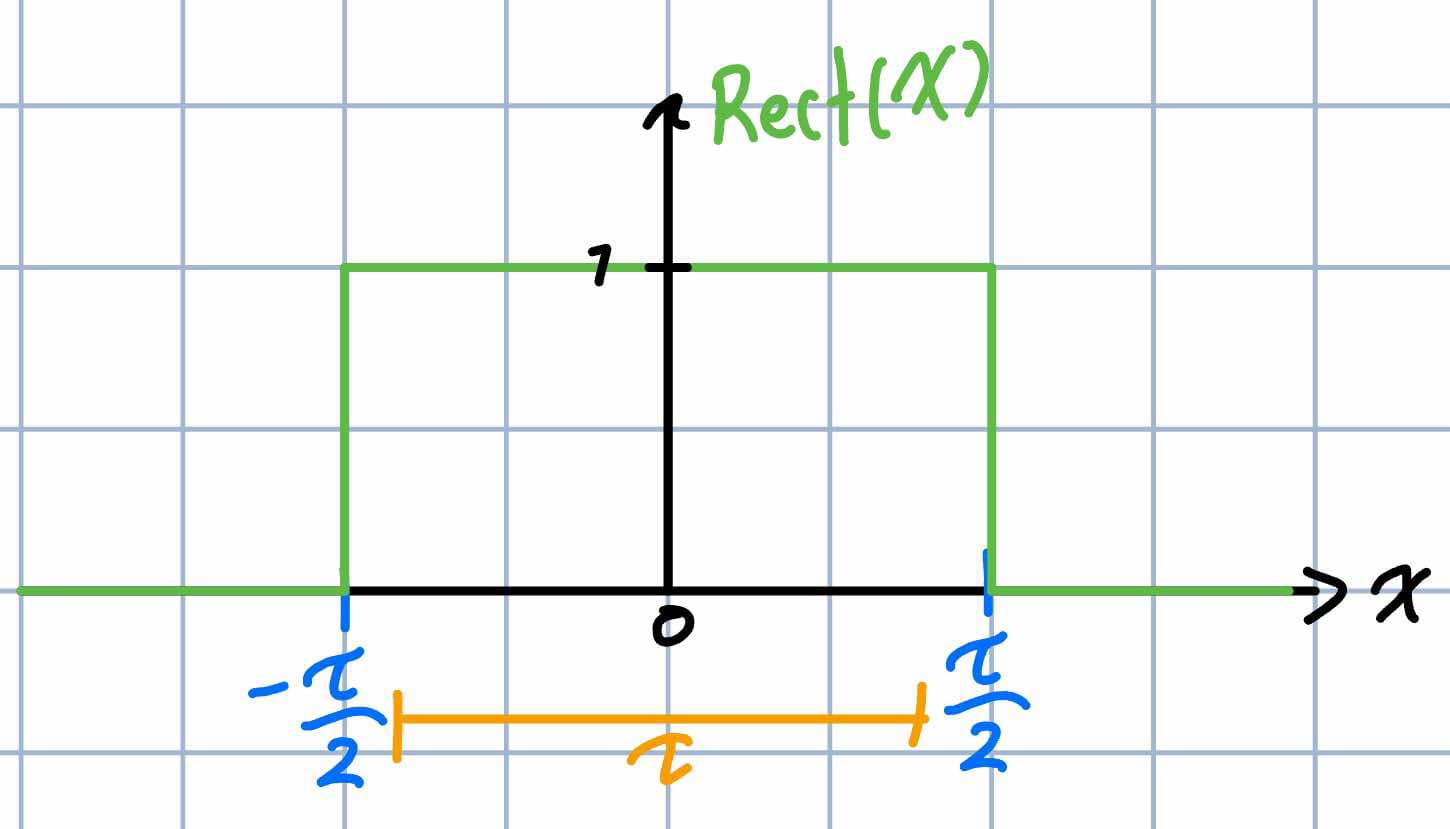
\includegraphics[width=0.4\textwidth]{images/ch4/pulse_rectangulaire.jpg}
    \caption{Pulse rectangulaire de hauteur 1}
    \end{figure}

Par (3.3), 

\begin{equation*}
    c(\omega) = \frac{1}{2\pi}\int_{-\infty}^{\infty}\text{Rect}(x)e^{-i\omega x}dx = \frac{1}{2\pi}\int_{-\tau/2}^{\tau/2}e^{-i\omega x}dx = \frac{1}{2\pi}\int_{-\tau/2}^{\tau/2}\left(\cos(\omega x) - i\sin(\omega x)\right)dx
\end{equation*}
\begin{equation*}
    = \frac{1}{2\pi}\left[\int_{-\tau/2}^{\tau/2}\underbrace{\cos(\omega x)}_\text{paire}dx - i\int_{-\tau/2}^{\tau/2}\underbrace{\sin(\omega x)}_\text{impaire}dx\right] = \frac{1}{\pi}\int_{0}^{\tau/2}\cos(\omega x)dx = \frac{1}{\pi \omega}\sin(\frac{\tau\omega}{2})
\end{equation*}

Si on pose $\tau = 1$ à des fins de représentation, on peut voir de quoi à l'air $c(\omega)$ dans cet exemple.

\begin{figure}[H]
    \centering
        
\includegraphics[width=0.6\textwidth]{images/ch4/coeff_pulse_rectangulaire.png}
    \caption{$c(\omega)$ pour le pulse rectangulaire ($\tau = 1$)}
    \end{figure}

Par (3.2),

\begin{equation*}
    \text{Rect}(x) = \int_{-\infty}^{\infty}\frac{\sin(\frac{\tau\omega}{2})}{\pi \omega}e^{i\omega x}d\omega
\end{equation*}

Pour vérifier que cela tient, il faudrait évaluer l'intégrale, ce qui à priori ne semble pas simple du tout. Si on approximait l'intégrale (en prenant par exemple des bornes d'intégration qui tendent progressivement vers $-\infty/\infty$), on verrait graphiquement qu'on retomberait bien sur la figure 6.

\subsection{Exponentielle décroissante symétrique}
Soit la fonction exponentielle décroissante symétrique $f(x) = Ae^{-B\abs{x}}$ où $A \in \mathbb{R}$ et $B \in \mathbb{R}_{> 0}$ sont des constantes.

\begin{figure}[H]
    \centering
        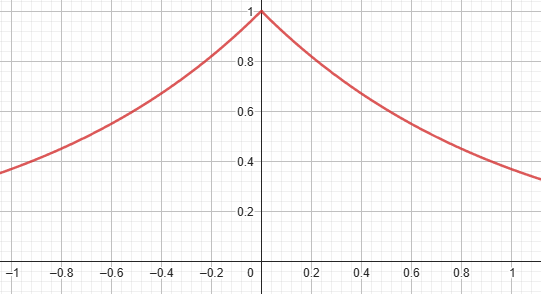
\includegraphics[width=0.45\textwidth]{images/ch4/expo_decroissante_sym.png}
    \caption{La fonction exponentielle décroissante symétrique ($A=1, B=1$)}
    \end{figure}

Par (3.3), on trouve 

\begin{equation*}
    c(\omega) = \frac{1}{2\pi}\int_{-\infty}^{\infty}Ae^{-B\abs{x}}e^{-i\omega x}dx = \frac{A}{2\pi}\left[\int_{-\infty}^{0}e^{Bx}e^{-i\omega x}dx + \int_{0}^{\infty}e^{-Bx}e^{-i\omega x}dx\right]
\end{equation*}
\begin{equation*}
    = \frac{A}{2\pi}\left[\frac{e^{(B-i\omega)x}}{B - i\omega}\eval{}_{-\infty}^{0} - \frac{e^{-(B+i\omega)x}}{B + i\omega}\eval{}_{0}^{\infty}\right] = \frac{A}{2\pi}\left[\frac{1}{B-i\omega} + \frac{1}{B+i\omega}\right] = \frac{A}{2\pi}\frac{(B+i\omega) + (B-i\omega)}{(B-i\omega)(B+i\omega)} = \frac{AB}{\pi(B^2+\omega^2)}
\end{equation*}

\begin{figure}[H]
    \centering
        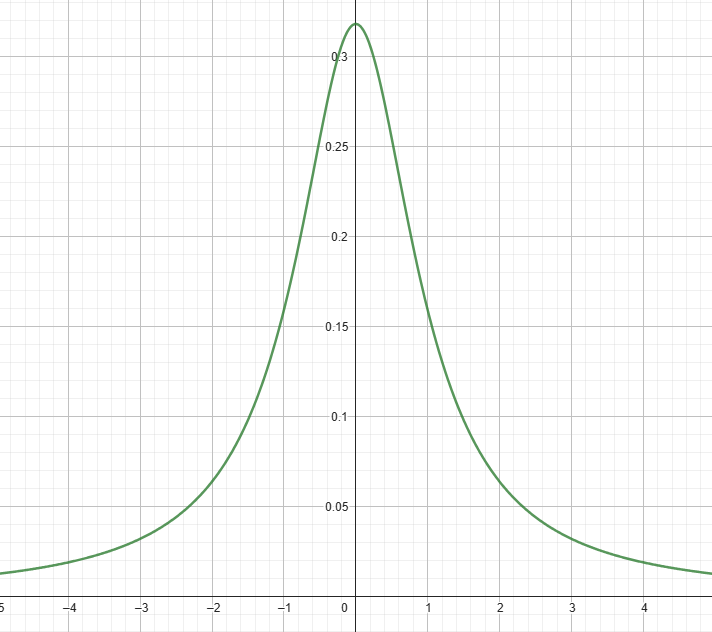
\includegraphics[width=0.35\textwidth]{images/ch4/coeff_expo.png}
    \caption{$c(\omega)$ pour la fonction exponentielle décroissante symétrique ($A=1, B=1$)}
    \end{figure}

Par (3.2), on a

\begin{equation*}
    f(x) = Ae^{-B\abs{x}} = \int_{-\infty}^{\infty}\frac{AB}{\pi(B^2+\omega^2)}e^{i\omega x}d\omega
\end{equation*}

dont on peut montrer que l'intégrale redonne bien l'exponentielle décroissante symétrique.

\subsection{Fonction boîte}
Similaire au pulse rectangulaire, on définit la fonction boîte comme 

\begin{equation*}
    B_k(x) = \begin{cases}
        1/k & \text{si } \abs{x} < k/2 \\
        0 & \text{sinon}
    \end{cases}    
\end{equation*}

\begin{figure}[H]
    \centering
        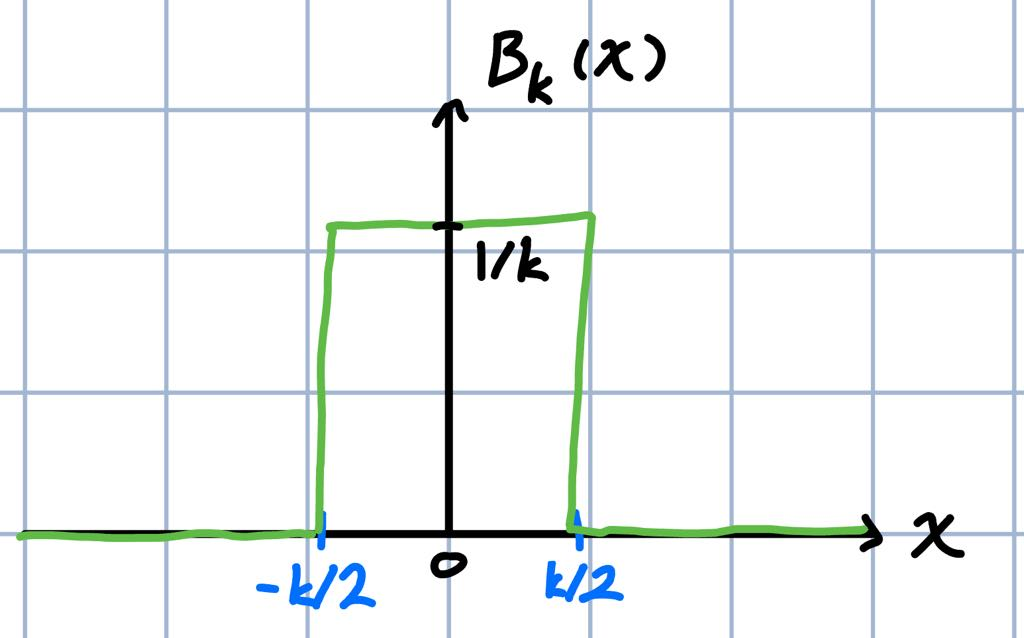
\includegraphics[width=0.35\textwidth]{images/ch4/fct_boite.jpg}
    \caption{La fonction boîte $B_k(x)$}
    \end{figure}

Tout de suite, on remarque que l'aire de la fonction boîte vaut 1 $\forall k >0$, c'est-à-dire que $\int_{-\infty}^{\infty}B_k(x)dx = 1 \ \forall k > 0$. Le calcul de sa transformée de Fourier se fait assez facilement sachant qu'on a déjà calculé la transformée de Fourier pour le pulse rectangulaire. En effet, on a qu'à remplacer $\tau$ par $k$ et multiplier le tout par $\frac{1}{k}$. Ainsi, 

\begin{equation*}
    c(\omega) = \frac{1}{\pi k \omega}\sin(\frac{k\omega}{2})
\end{equation*}

et 

\begin{equation*}
    B_k(x) = \int_{-\infty}^{\infty}\frac{1}{\pi k \omega}\sin(\frac{k\omega}{2})e^{i\omega x}d\omega
\end{equation*}

qui tiennent pour les mêmes raisons que dans le cas du pulse rectangulaire.

\subsection{Delta de Dirac}
% Le delta de Dirac $\delta(x)$ est une fonction nulle partout sauf à l'origine et dont $\int_{-\infty}^{\infty}\delta(x)dx = 1$. Avec ce qu'on vient de voir à la précédente sous-section, on peut dire que 

% \begin{equation*}
%     \delta(x) = \lim_{k \rightarrow 0} B_k(x)
% \end{equation*}

% Alors, on a simplement à réutiliser nos trouvailles pour la fonction boîte et regarder cela dans la limite où $k \rightarrow 0$. Ainsi,

